 \documentclass[a4paper]{jpconf}
\usepackage{graphicx}
\usepackage{booktabs}
\usepackage{siunitx}
\usepackage{enumitem}
\usepackage[utf8]{inputenc}
\usepackage{csquotes}
\usepackage[backend=biber,style=authoryear]{biblatex}

\usepackage{subfig,multicol}
\usepackage[export]{adjustbox}
\usepackage{float}

\usepackage[english]{babel}
\usepackage{fancyhdr}

\usepackage{lastpage}
\pagestyle{fancy}
\fancyhf{}
\rfoot{Page \thepage \hspace{1pt} of \pageref{LastPage}}


\addbibresource{Congested.bib}
%\nocite{*}




\begin{document}
\title{Towards a city congestion index: methodological explorations using Google's Distance Matrix API}

\author{Jonathan Cohen and Jorge Gil}

\address{Chalmers University of Technology, Sven Hultins gata 6, SE-412 96, Göteborg, Sweden}

\ead{jonathan.cohen@chalmers.se}




\begin{abstract}
	Sustainable transport systems are a necessary requirement to achieve efficient economic performance, enhance urban quality of life and diminish environmental costs. Congestion, a negative externality of mobility, is responsible for urban pollution, inefficiency and has adverse effects over individuals facing this problem. For these reasons, transport and city planning agencies have developed interests in defining and measuring transportation congestion. Although, different definitions and metrics have been used, congestion measurements are found aggregated at a city level or for particular road segments. This study proposes a methodology that produces information from a web traffic service to map traffic congestion within an urban area. The method is simple and generalizable enough to be adopted in different urban areas. This paper presents the analysis of four european cities (Amsertdam, Glasgow, Goteborg and Lisbon) and show that the conclusions are consistent with the results obtained from internationally recognized organizations such as INRIX and TomTom.
\end{abstract}


\section{Introduction}%%%%%%%%%%%%%%%%%%%%%%%%%%%%%%%%%%%%%%%%%%%%%%%%%%%
%%%%%%%%%%%%%%%%%%%%%%%%%%%%%%%%%%%%%%%%%%%%%%%%%%%%%%%%%%%%%%%
\indent Although United Nations (UN) has not identified  efficient, clean and equitable mobility as one the 18 Sustainable Development Goals (SDGs), transportation indicators are present within several Goals (CITE UN SDGS). Sustainable transport systems are acknowledged to be necessary pre-conditions to enhance socio-economic opportunities, diminish environmental costs and improve road safety conditions (CITE IMPORTANCE OF TRANSPORT). \par
\indent Within cities over 60\% of the total wealth is produced and the positive externalities of living in urban areas has been extensible registered. However, as the population density increases a set of negative externalities such as pollution, crime or congestion erode the benefits of urban life (UN - OECD). \par

\indent The definition of congestion in transportation facilities has evolved over the years (XXXXXXX) and there is no universal accepted definition for the problem. According to LOMAX 1997, different actors are interested in understanding different parts of traffic congestiom; depending on the what the objective of the study is, different definitions can be adopted and as a result different measurments used. 

\indent In a survey deployed to reveal the importance of traffic congestion, (Bertini, 2005) shows the different approaches that can be taken to define an measure congesiotn. The results reinforce the idea that multiple definitions co-exist and that they can be used for different purposes

\indent In this paper traffic congestion in cities will be considered a \textit{'by-product of their success in attracting people to jobs and other amenities, and the inability of cities to improve/expand transportation capacity to keep pace with this growth.'} (Falcocchio \& Levinson, 2015) continue stating that \textit{'the cities’ challenge is to keep congestion manageable as their population and economies grow. To be helpful in congestion management decisions, the definition of congestion should be based on a comparison of “actual travel times” with “expected travel times” for peak hour and off-peak conditions.'}


\subsection{Research Aim}%%%%%%%%%%%%%%%%%%%%%%%%%%%%%%%%%%%%%%%%%%%%%
\indent As mentioned above, traffic congestion is an urban problem that deteriorate the positive benefits of urban life, therefore is imperative to understand the problem in depth and look at it from different angles. Traditional congestion measurements are found to be costly and through practice or research different methods have been explored to overcome this issue. \par
\indent One avenue of research understands congestion as a time and location specific problem, which occurs in a road segment and that its consequences are suffered from those in the immediate surroundings. A second understanding of the problem deals with the individuals who are affected by traffic. \par
\indent Focusing on this second interpretation of the problem, the aim of this research is to provide a methodology to spatialize congestion to expose how traffic congestion is distributed across an urban area. The map of congestion can provide useful information to local authorities and planners since more disaggregated spatial information will be provided. \par


\section{Theoretical Background} %%%%%%%%%%%%%%%%%%%%%%%%%%%%%%%%%%%%%%%%%%%%%
%%%%%%%%%%%%%%%%%%%%%%%%%%%%%%%%%%%%%%%%%%%%%%%%%%%%%%%%%%%%%%%%%%%%%%%%% 
\indent Congestion definitions can be categorized into the following groups
\subsection{Traffic congestion measurements}
\indent What congestion indices exist out there? 


\subsection{Characteristics of the metric}
\indent 


\subsection{Data collection}


\indent Depending on the 
how is congestion defined. by one or two authors only.


The components of congestion: the route between OD pair, the distance and travel time (consequently, the speed of travel), the capacity of the route. inherently a travel time difference problem.
The components of a broader understanding of the phenomenon: a person travelling with a purpose, a date and time of day, two locations (origin and destination). This brings it closer to definitions of accessibility, but measuring the convenience of travel (refs on this?)
\indent What congestion indices exist out there? \par
How it is measured (absolute and relative indices)

\indent Practice/literature\par


\indent How are others mapping congestion (or real travel time) with geodata? (edited) \par
The focus on the link (flow and speed), the focus on visualisation.





\indent As the list of traffic congestion indicators
As the list of 
At the same time new methodologies to measure traffic congestion were developed, researchers 


At the same time different 

some researcher were 

For instance in Lomax (1993) 

In parallel, as the list of traffic congestion measurements increased 










\section{Methodology} %%%%%%%%%%%%%%%%%%%%%%%%%%%%%%%%%%%%%%%%%%%%%%%%%% %%%%%%%%%%%%%%%%%%%%%%%%%%%%%%%%%%%%%%%%%%%%%%%%%%%%%%%%%%%%%%%%%%%%%
\indent At its core the methodology described in this section details a process of collecting and processing data from an internet service that provides traffic estimations and routing optimization. The method presented here correspond to data extracted from the Distance Matrix API form Google Inc., but the exact same exercise could be done with other services such as HERE or TOMTOM.\par
\indent Given the quantity and nature the methodology that will be described above, was coded and executed using R in Rstudio and the functions written can be found in GitHub. \par
\indent In order to prioritize clarity over narrative, the necessary steps followed by this methodology are listed below: 
\begin{enumerate}[label=\arabic*)]
	\item Select and define an urban area to work with: After an urban area is selected a synthetic boundary needs to be drawn. In this case, for simplicity reasons, a circular buffer zone was used to define the 'study area'.
	\item Choose a zoned cartography of the area and clip it accordingly to the boundaries: Choose from any geographical authority a zoned cartography. Census tracks, neighbourhoods or plots can be chosen. In our case the European Population grids was selected.	
	\item Make centroids from the zones and extract the geographical position of each point
	\item Generate permutations from centroids to create an empty Origin-Destiny Matrix: Using the GPS location (latitude and longitude) of each centroid, a list of all possible combinations is generated (a total of n*(n-1) routes).  For instance, is the area to be studied contains 3 areas (A, B \& C), the OD matrix will consider the following routes: (i) A to B, (ii) A to C, (iii) B to A, (iv) B to C, (v) C to A \& (vi) C to B. 
	\item Define a \textit{congested} and \textit{non-congested} times: Using the difference between a \textit{congested} and \textit{non-congested} situation as the definition of congestion, a time need to be specified. As information from Google will be used, a future time needs to be specified. Based on previous results, Thursday, October 15, 2020 8:30:00 AM was chosen as a \textit{congested} moment and Wednesday, July 15, 2020 3:30:00 AM, as a \textit{non-congested}.
	\item Use a routing service to estimate time and distance travelled: The origin to destination list with the \textit{congested} and \textit{non-congested} time specification were used as inputs for the routing service to estimate travel time and distance. 
	\item Calculate descriptive statistics and visualize: Histograms, scatter plots and descriptive statistics were calculated to detect possible  problems such as missing data or outliers. 
	\item Deal with data issues: As the centroid of the polygon based on the European Population Grid could fall over a problematic place such as river, park or railway lot (places where google maps cannot match an address), some routes could not be retrieved and consequently were left out of the study.
	\item Calculate KPIs: Based on research done in the past the following can be derived:
		\begin{itemize}
			\item Time difference:	
			\item Travel Time Index (TTI):			
		\end{itemize}	
	\item Aggregate data generated and join to spatial grid: With the data retrieved averages by the origins were calculated and joined to these values joined to the original zoned urban area. 
	\item Calculate descriptive statistics and visualize: The results at the Grid level are analyzed using descriptive statitics and basic plotting. This step can be seen as check-up point that can contribute to identify data anomalies such as missing data or outliers. 
	\item Map the results: Finally, once the data clean-up process is done, a map with the processed variables can be generated.
\end{enumerate}

\indent To demostrate how the method could be used in practice, four European cities where selected as a proof of concept.\par

%%%%%%%%%%%%%%%%%%%%%%%%%%%%%%%%%%%%%%%%%%%%%%%%%%%%%%%%%%%%%%%%%%%%%%%%
\section{Data} %%%%%%%%%%%%%%%%%%%%%%%%%%%%%%%%%%%%%%%%%%%%%%%%%%%%%%%%%
%%%%%%%%%%%%%%%%%%%%%%%%%%%%%%%%%%%%%%%%%%%%%%%%%%%%%%%%%%%%%%%%%%%%%%%%
\indent In order to run the analysis for a desired urban area, a zoned cartography of the area is needed. In this opportunity, as a proof of concept the 1km2 population grid from the EuroStat (GEOSTAT 2011) was used. Amsterdam, Glasgow, Goteborg and Lisbon were selected and from their historical centre a buffer zone was used to delimit the \textit{city} boundary. The geographic coordinates of the centroid of each 1km2 square was used to create the list of all possible routes. \par
\indent From these list of origins a synthetic Origin-Destiny matrix was created: all possible origins to all possible destinations was then used to retrieve data for a \textit{congested} and \textit{non-congested} moments. 

\subsection{Data retrieved} %%%%%%%%%%%%%%%%%%%%%%%%%%%%%%%%%%%%%%%%%%%%
%%%%%%%%%%%%%%%%%%%%%%%%%%%%%%%%%%%%%%%%%%%%%%%%%%%%%%%%%%%%%%%%%%%%%%%%
The process generates information for a total n*(n-1) routes (n being the number of zones). For instance, Lisbon is divided into 119 squares and the number of possible routes is 119*118 = 14,042 (then 28,084 travels were estimated). Amsterdam has 131 zones, Glasgow 136 and Goteborg 123 (17,030, 18,360 and 15,006 routes respectively). A summary of the descriptive statistics for the time in minutes can be found in Table \ref{tab:Results_routes}.

\begin{table}[ht]		
	\centering
	\begin{tabular}{rlrrrrr}
		\hline
		& Congested scenario (mins) & Routes & Mean & S.D. & Min & Max 	   \\ 
		\hline
		1 & Amsterdam 	& 17,023 & 20.26 & 6.86 	& 0.65 & 48.57 		   \\ 
		2 & Glasgow 	& 18,355 & 23.08 & 8.68 	& 1.42 & 56.88 		   \\ 
		3 & Goteborg 	& 14,997 & 18.01 & 6.82 	& 1.37 & 57.97 	       \\ 
		4 & Lisbon 		& 14,043 & 28.16 & 11.70 	& 1.37 & 84.63 	       \\ 
		
		\hline
		& Non-Congested scenario & Routes & Mean & S.D. & Min & Max    \\ 
		\hline
		1 & Amsterdam	& 17,023 & 11.70 & 3.71 & 0.52 & 24.90 	       \\ 
		2 & Glasgow 	& 18,355 & 11.93 & 3.99 & 0.83 & 24.85 	       \\ 
		3 & Goteborg 	& 14,997 & 13.09 & 5.29 & 1.10 & 49.18 	       \\ 
		4 & Lisbon 		& 14,043 & 12.82 & 5.77 & 0.77 & 46.90         \\ 
		\hline
	\end{tabular}
	\caption {Descriptive Statistics of travel times by city}
	\label{tab:Results_routes}
\end{table}

\indent The amount of route information retrieved is consistent with the amount of zones in the city and as expected, the \textit{congested} situation on average takes longer time. Formally an independent-samples t-test was conducted to compare the travel times under a \textit{congested} and \textit{non-congested} situations. For each city, the time difference was found statistically significant with a confidence level of 99\%.

%%%%%%%%%%%%%%%%%%%%%%%%%%%%%%%%%%%%%%%%%%%%%%%%%%%%%%%%%%%%%%%%%%%%%%%%
\section{Results} %%%%%%%%%%%%%%%%%%%%%%%%%%%%%%%%%%%%%%%%%%%%%%%%%%%%%%
%%%%%%%%%%%%%%%%%%%%%%%%%%%%%%%%%%%%%%%%%%%%%%%%%%%%%%%%%%%%%%%%%%%%%%%%
After capturing, processing and aggregating the data obtained from the API, table \ref{tab:Results_grids} on page ~\pageref{tab:Results_grids} contains the descriptive statistics for time difference and TTI. In this case, the number of observations corresponds to the number of zones in the map and each zone holds the mean of all the trips departed from that origin. 
\indent The results show that the methodology successfully captured diversity between cities. For instance, in Lisbon the average time difference is of 15.3 mins, with a maximum of 21.6 mins, meanwhile in Goteborg on average delays are of 4.9 mins with a maximum of 8 mins.  

\begin{table}[ht]		
	\centering
	\begin{tabular}{rlrrrrr}
		\hline
		  & Time Difference (mins) & Zones & Mean & S.D. & Min & Max \\ 
		\hline
		1 & Amsterdam 	& 131 	& 8.57  & 2.39 & 5.38 & 19.03 \\ 
		2 & Glasgow 	& 136 	& 11.15 & 1.88 & 7.66 & 15.64 \\ 
		3 & Goteborg 	& 123 	& 4.92  & 0.99 & 3.22 & 8.06  \\ 
		4 & Lisbon 		& 119 	& 15.34 & 2.67 & 9.74 & 21.57 \\ 
		
		\hline
		  & TTI	& Zones & Mean & S.D. & Min & Max \\ 
		\hline
		1 & Amsterdam 	& 131 & 1.74 & 0.23 & 1.36 & 2.61 \\ 
		2 & Glasgow 	& 136 & 1.94 & 0.14 & 1.60 & 2.31 \\ 
		3 & Goteborg	& 123 & 1.38 & 0.09 & 1.21 & 1.69 \\ 
		4 & Lisbon 		& 119 & 2.21 & 0.16 & 1.70 & 2.57 \\ 
		\hline
	\end{tabular}
	\caption {Aggregated descriptive statistics by zones}
	\label{tab:Results_grids}
\end{table}

\indent Although, the table above reveals relevant insights about these cities, local authorities or planners would not know which places or who is being affected by traffic congestion. Therefore, in figure \ref{fig:result_tti} the TTI for each city was mapped. By looking at these maps several conclusions about where and how bad congestion is across the city. For instance, in all four cities, although the historical centre is the nearest point to all other destinations, when congestion is taken into account, these places face the highest TTI. This indicates that in a \textit{non-congested} situation, the city centre is highly accessible but when \textit{congested}, the advantage of being central gets eroded. \par
\indent These maps also show that the methodology presented in this study 
was able to capture differences across cities successfully. In Goteborg, the historical city centre gets mainly congested, meanwhile the other parts of the city remain with similar levels of congestion. In Lisbon, traffic congestion is more scattered across the city, presenting islands of low congestion (where the CBD and commercial areas have moved to).


\begin{figure}[H]
	\centering
	\begin{multicols}{2}
		\noindent
		%
		\subfloat[Amsterdam]{\centering
			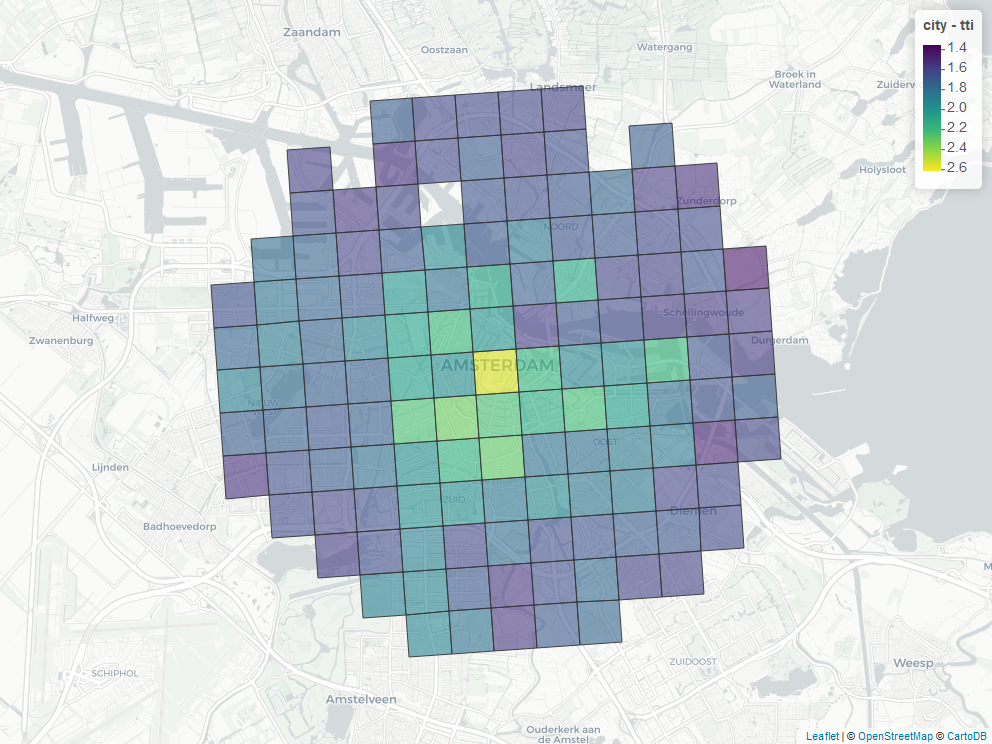
\includegraphics[width=0.8\linewidth, height=4cm]{./Img/amsterdam_tti}} \par 
		%
		\subfloat[Glasgow]{\centering
			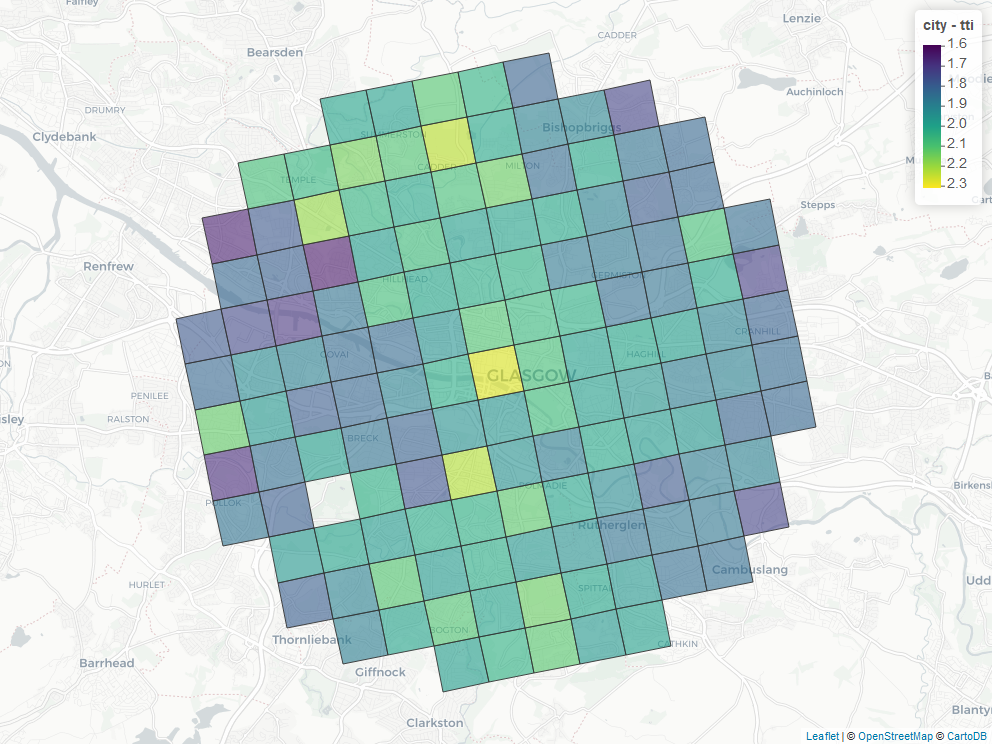
\includegraphics[width=0.8\linewidth,height=4cm]{./Img/glasgow_tti}} \newpage
		%
		\subfloat[Goteborg]{\centering
			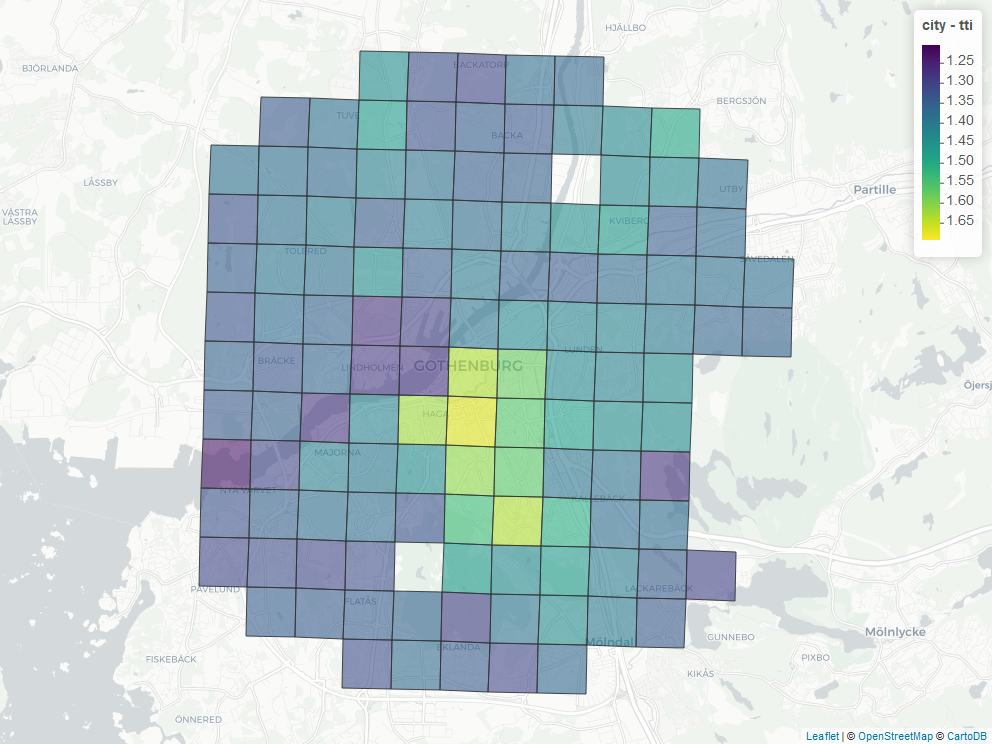
\includegraphics[width=0.8\linewidth,height=4cm]{./Img/goteborg_tti}} \par
		%
		\subfloat[Lisbon]{\centering
			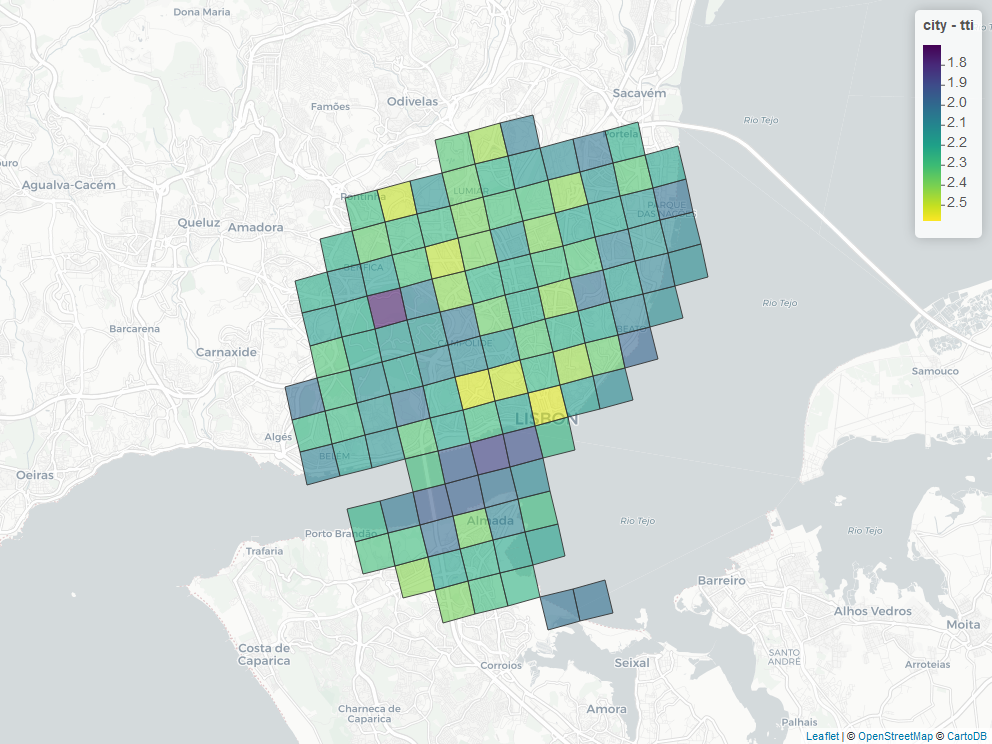
\includegraphics[width=0.8\linewidth, height=4cm]{./Img/lisbon_tti}} \par
		%	
	\end{multicols}
	\caption{Images extracted from results}
	\label{fig:result_tti}
\end{figure}


\begin{figure}[H]
	\centering
	\begin{multicols}{2}
		\noindent
		%
		\subfloat[Amsterdam]{\centering
			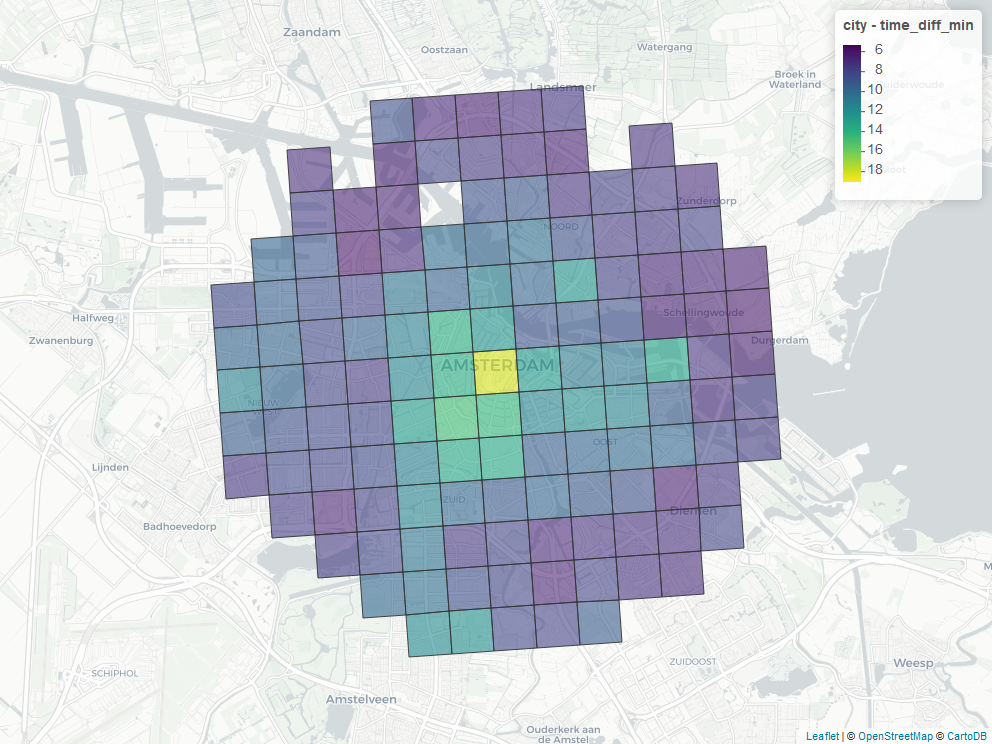
\includegraphics[width=0.8\linewidth, height=4cm]{./Img/amsterdam_time_diff_min}} \par 
		%
		\subfloat[Glasgow]{\centering
			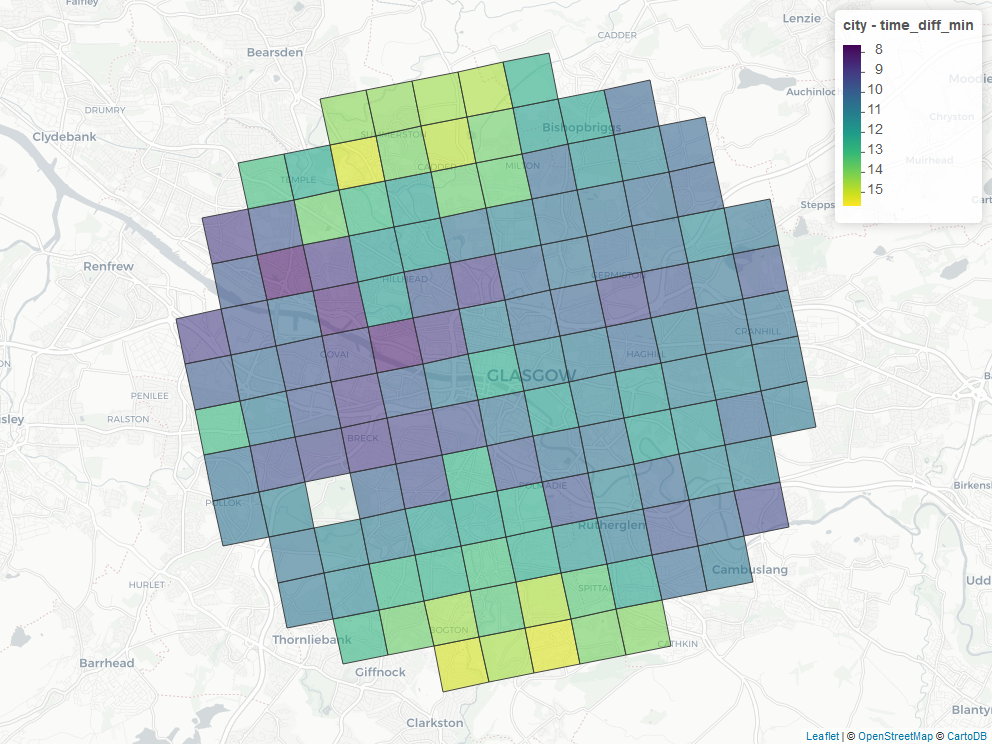
\includegraphics[width=0.8\linewidth,height=4cm]{./Img/glasgow_time_diff_min}} \newpage
		%
		\subfloat[Goteborg]{\centering
			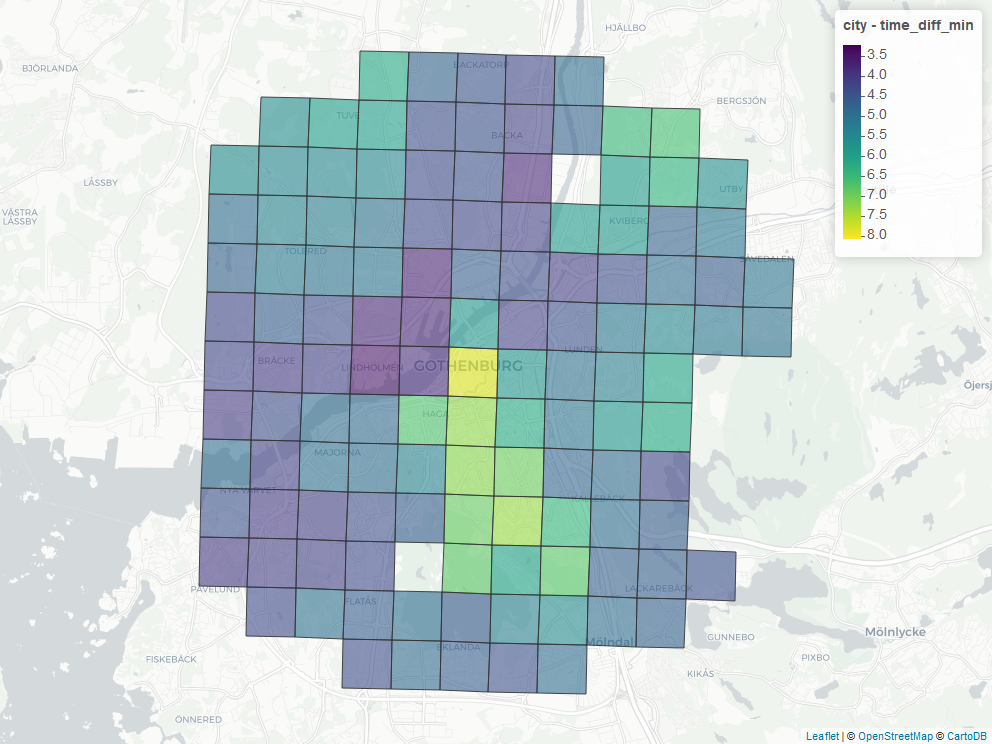
\includegraphics[width=0.8\linewidth,height=4cm]{./Img/goteborg_time_diff_min}} \par
		%
		\subfloat[Lisbon]{\centering
			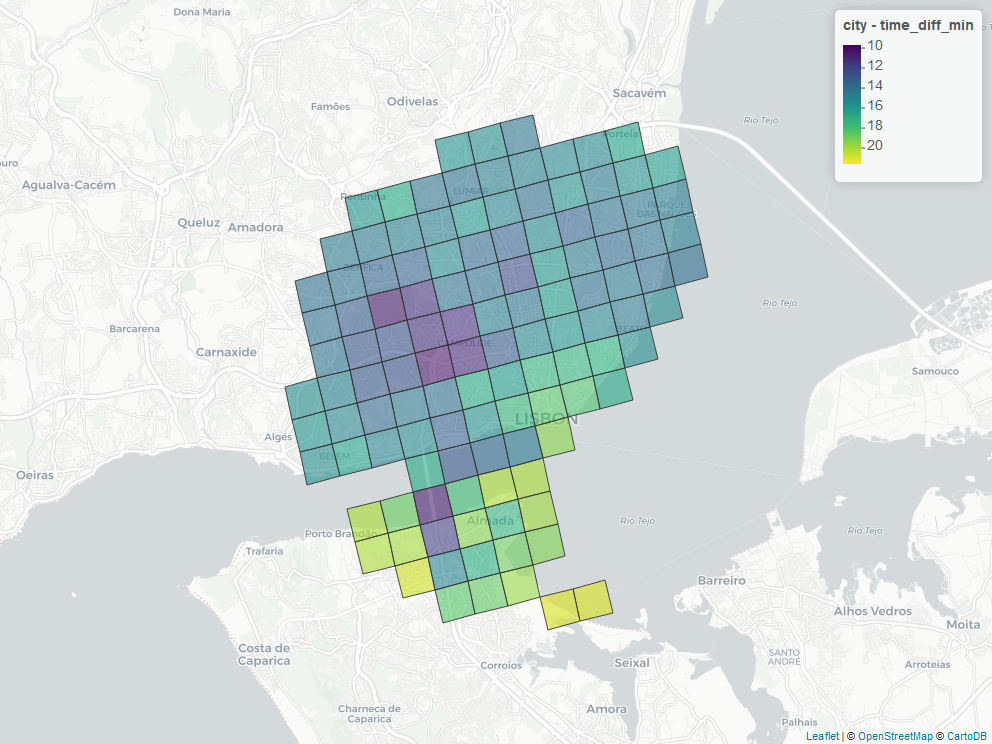
\includegraphics[width=0.8\linewidth, height=4cm]{./Img/lisbon_time_diff_min}} \par
		%	
	\end{multicols}
	\caption{Images extracted from results}
	\label{fig:result_diff}
\end{figure}


%%%%%%%%%%%%%%%%%%%%%%%%%%%%%%%%%%%%%%%%%%%%%%%%%%%%%%%%%%%%%%%%%%%%%%%%
\section{Discussion}, %%%%%%%%%%%%%%%%%%%%%%%%%%%%%%%%%%%%%%%%%%%%%%%%%%%
%%%%%%%%%%%%%%%%%%%%%%%%%%%%%%%%%%%%%%%%%%%%%%%%%%%%%%%%%%%%%%%%%%%%%%%%
\indent The methodology presented in this paper exploits a new data source to provide spatial insights about traffic congestion in different cities. The information generated allows planning and transport agencies to reconstruct some of the most popular indexes discussed in the theoretical background section.\par

\indent With completely different business models, INRIX, HERE and TomTom are two internationally known companies which in the last years started to offer similar transportation insights as a service. Historically, INRIX has been consulted to provide he levels of congestion in several countries in the OECD and U.S. transport agencies, but given the increase in the amount of devices embedded with GPS, other businesses have found them self in a position of exploiting these new data sources. Nowadays, they all offer transportation consulting services. INRIX and TomTom publish reports of traffic congestion and rank cities according to different criteria. [SHOULD WE SHOW A A GRAPH WITH THIS?] The aggregated results producing this methodology are consistent with those produced by both companies. Moreover, the methodology proposed in this paper allows practitioners to visualize how congestion is spatially distributed across the city.\par

\indent The results presented here, took the EuroStat population 1km2 grid cell to retrieve traffic information. Certainly, this decision was arbitrary and the shape/size of these areas can be subject of debate. Nevertheless, the zones used for the analysis can be easily interchanged allowing the process to be enriched.\par

\indent Traffic congestion deteriorate different domains of urban life and as a consequence the focus on the problem varies across disciplines. The maps of congestion produced as a result of applying this methodology can be used to understand who suffers from congestion the most and what parts of the city are more vulnerable to the problem. This approach can be iterated over time, to see how transport congestion evolves over the city and evaluate to what extent certain policies are being effective in changing traffic congestion patterns.\par

\subsection{Examples to cite} %%%%%%%%%%%%%%%%%%%%%%%%%%%%%%%%%
\indent As shown
 1.\cite{Lomax1997} \par
 2.\parencite{Lomax1997} \par 
 3.\textcite{Lomax1997} \par


\subsection{Limitations and future work}
\indent The methodology presented in this study relays primarily in Google's web service and this fact is a drawback as users have no control over the service standards, usability or costs. For instance, the type request performed during this study had a cost of 10 U\$D/1000 requests, considering a grid of 100 areas, will generate 9,900 travel routes and to estimate congestion a total of 19,800 requests will be needed. This process will involve a cost of 198 U\$D. This issue relates with future avenues of research which involve  exploring other data sources and comparing them.\par

\indent This process was not conceived to show congestion levels at street level, but to identity areas which area affected by this phenomena. Transport or planning practitioners interested in getting traditional information about levels of service, will not find answers by applying this methodology. \par 

\indent The results presented here, do not necessarily imply that \textit{'more congested'} places are demanding for solutions from public administration, but attention. \textit{'Traffic problems'} can be the result of poor infrastructure, an excess of demand or a combination of both. The method only reflects time delays faced by private commuting and in some cases, such as in city centres, this can be a desirable tool to demotivate car use.\par

\indent The population grid was used because it allows to eventually weight the results obtained. Instead, other commonly used cartography could be used. Census tracks with socio-economic information could be used to refine the method, the amount of cars or age groups could help to better understand to what degree this citizens are affected and to explore whether there is a relation between car use and congestion levels. Moreover, an origin and destination survey with geographical zones can be used used in the study to weight the different desire lines of travel. Depending on the characteristics of each data source, this methodology can be expanded and refined in different manners.

\indent Finally, but not least Google API also offers estimations for public transport that depending on the city can be also used to estimate the costs of moving thought the city. 



\subsection{Applications}
\indent As shown \cite{Lomax1997} Traffic congestion measurements can be used  


\subsection{Limitations and future work}
\indent Grid size and costs
In this case 


\indent Weights
using population
using an OD matrix

1km grid size can be too coarse for spatial planning, has impact o

\indent use census tracks or population statistics to correlate with socio-demographics


\indent Reviewer Remarks:This is a very interesting paper proposal. It will be interesting to learn how the impact of different types of car engines (petrol, diesel, electric, etc) will impact CO2 emissions in congested and non-congested traffic flows.

%%%%%%%%%%%%%%%%%%%%%%%%%%%%%%%%%%%%%%%%%%%%%%%%%%%%%%%%%%%%%%%%%%%%%%%%
\section{Conclusion} %%%%%%%%%%%%%%%%%%%%%%%%%%%%%%%%%%%%%%%%%%%%%%%%%%%
%%%%%%%%%%%%%%%%%%%%%%%%%%%%%%%%%%%%%%%%%%%%%%%%%%%%%%%%%%%%%%%%%%%%%%%%
\indent The study presented a methodological approach to study the how traffic congestion is spatially distributed within an urban area. Generating a synthetic Origin-Destiny matrix, the method uses an online routing service to estimate different travel routes. The methodology provides a non-expensive, generalizable and systematic to estimate congestion in different parts of a city. The data retrieved can be mapped, thus used by city planners and transportation agencies. The aggregation of the data provide conclusions that are consistent with internationally recognized institutions such as INRIX and TomTom. 


%%%%%%%%%%%%%%%%%%%%%%%%%%%%%%%%%%%%%%%%%%%%%%%%%%%%%%%%%%%%%%%%%%%%%%%%
\printbibliography %%%%%%%%%%%%%%%%%%%%%%%%%%%%%%%%%%%%%%%%%%%%%%%%%%%%%
%%%%%%%%%%%%%%%%%%%%%%%%%%%%%%%%%%%%%%%%%%%%%%%%%%%%%%%%%%%%%%%%%%%%%%%%


\end{document}








